\documentclass[margin=1mm]{standalone}
\usepackage[utf8]{inputenc}
\usepackage{amsmath}
\usepackage{amsfonts}
\usepackage{amssymb, bm}
\usepackage{tikz}
\usetikzlibrary{calc,arrows,positioning,shapes,shapes.gates.logic.US,trees, backgrounds}
\usetikzlibrary{fit, positioning}

\begin{document}
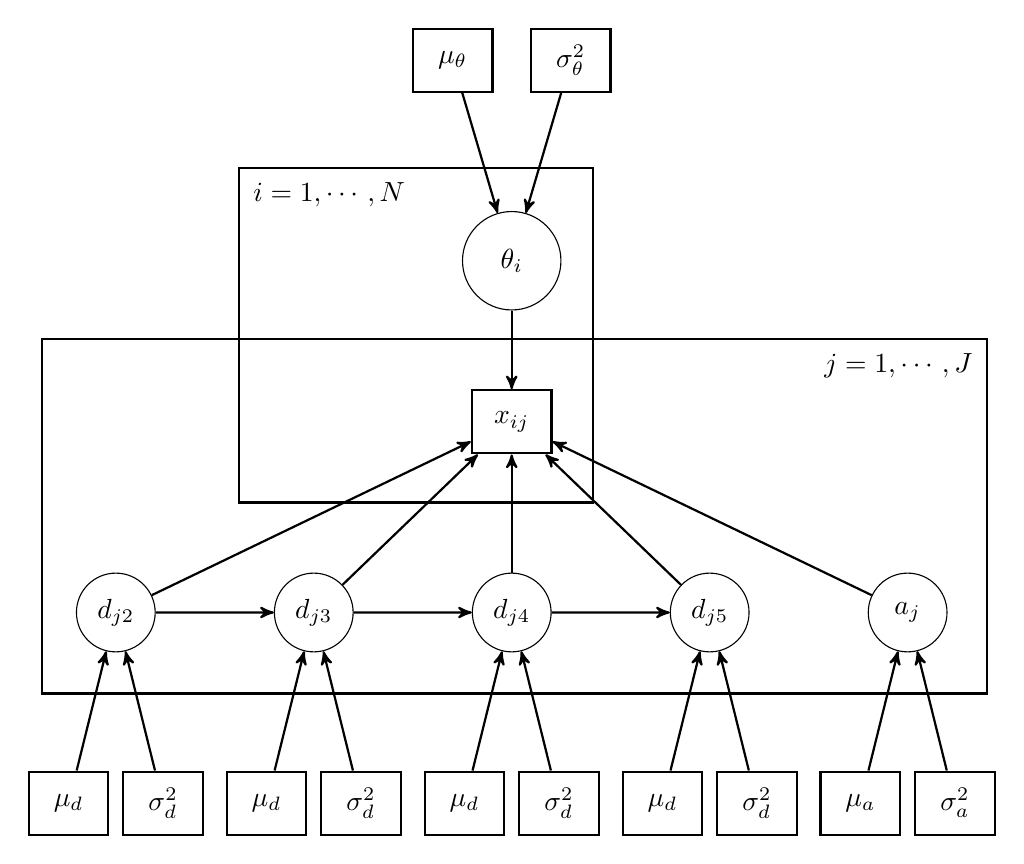
\begin{tikzpicture}[auto,scale=3,
	latent/.style={circle,draw,text badly centered, inner sep=2pt,minimum size=12.5mm},
	error/.style={circle,draw,text badly centered, inner sep=2pt,minimum size=10mm},
	manifest/.style={text centered, rectangle,draw,thick,inner sep=3pt,minimum height=8mm, minimum width=8mm, text width= 8 mm},
	  plate/.style={draw, shape=rectangle,thick, minimum height=4.25cm, minimum width=4.5cm, text width=1cm, align=right, inner sep=10pt, inner ysep=10pt, append after command={node[below right= 3pt of \tikzlastnode.north west] {#1}}},
	  plate2/.style={draw, shape=rectangle,thick, minimum height=4.5cm, minimum width=12cm, text width=1cm, align=right, inner sep=5pt, inner ysep=8pt, append after command={node[below left= 3pt of \tikzlastnode.north east] {#1}}},
	manifestRot/.style={text centered, rectangle, draw, thick,inner sep=3pt, minimum width=7mm, text width= 7mm, minimum height=15},
	manifestfront/.style={rectangle,draw,thick,inner sep=0pt,minimum size=12mm, fill=white},
	ghost/.style={rectangle, inner sep=0pt,text centered,    minimum height=0mm, minimum width=5mm, text width= 5 mm},
	lcorr/.style={<->,>=stealth', bend right=40},
	rcorr/.style={<->,>=stealth', bend left=40},
	fcorr/.style={<->,>=stealth', bend left=40},
	ofcorr/.style={<->,>=stealth', bend right=60},
	ofcorr2/.style={<->,>=stealth', bend left=60},
	intercept/.style={regular polygon,
        regular polygon sides=3,draw,thick,inner sep=0pt,minimum size=10mm},
	mean/.style={regular polygon,regular polygon sides=3,draw,thick,inner sep=0pt,minimum size=10mm},
	paths/.style={->, thick, >=stealth'},
	variance/.style={<->, thick, >=stealth', bend left=270, looseness=2},
	varianceTop/.style={<->, thick, >=stealth', bend right=270, looseness=2},
	unique/.style={<->, thick, >=stealth', loop below=270, looseness=8},
	factvar/.style={<->, thick, >=stealth', loop right=270, looseness=8}
	] % End Creating Path Model Pieces
\tikzset{mystyle/.style={->,double=black}}


% person model
\node [manifest] at (0,0) (x) {$x_{ij}$};
\node [latent]     [above = 1cm of x] (t) {$\theta_i$};
\node [manifest]   [above = 1.5cm of t,  xshift=-0.75cm] (mut)   {$\mu_{\theta}$};
\node [manifest]   [above = 1.5cm of t,  xshift= 0.75cm] (sigt)   {$\sigma^2_{\theta}$};
\node [error]      [below = 1.5cm of x] (dj4) {$d_{j4}$};
  \node [manifest] [below = 1.5cm of dj4, xshift=-.6cm] (dj40) {$\mu_{d}$};
  \node [manifest] [below = 1.5cm of dj4, xshift= .6cm] (dj41) {$\sigma^2_{d}$};  
\node [error]      [left = 1.5cm of dj4] (dj3) {$d_{j3}$};
  \node [manifest] [below = 1.5cm of dj3, xshift=-.6cm] (dj30) {$\mu_{d}$};
  \node [manifest] [below = 1.5cm of dj3, xshift= .6cm] (dj31) {$\sigma^2_{d}$};
\node [error]      [left = 1.5cm of dj3] (dj2) {$d_{j2}$};
  \node [manifest] [below = 1.5cm of dj2, xshift=-.6cm] (dj20) {$\mu_{d}$};
  \node [manifest] [below = 1.5cm of dj2, xshift= .6cm] (dj21) {$\sigma^2_{d}$};
\node [error]      [right = 1.5cm of dj4] (dj5) {$d_{j5}$};
  \node [manifest] [below = 1.5cm of dj5, xshift=-.6cm] (dj50) {$\mu_{d}$};
  \node [manifest] [below = 1.5cm of dj5, xshift= .6cm] (dj51) {$\sigma^2_{d}$};  
\node [error]      [right = 1.5cm of dj5] (aj) {$a_{j}$};
  \node [manifest] [below = 1.5cm of aj, xshift=-.6cm] (aj0) {$\mu_{a}$};
  \node [manifest] [below = 1.5cm of aj, xshift= .6cm] (aj1) {$\sigma^2_a$};

\node [plate={$i=1, \cdots, N$}] [right= -4cm of x, yshift=1.1cm] (p) {};
\node [plate2={$j=1, \cdots, J$}] [right= -6.5cm of x, yshift=-1.2cm] (p2) {};


% paths
\draw[paths] (t)  -- (x);
\draw[paths] (mut) -- (t);
\draw[paths] (sigt) -- (t);
\draw[paths] (aj) -- (x);
\draw[paths] (dj2) -- (x);
\draw[paths] (dj3) -- (x);
\draw[paths] (dj4) -- (x);
\draw[paths] (dj5) -- (x);
\draw[paths] (dj2) -- (dj3);
\draw[paths] (dj3) -- (dj4);
\draw[paths] (dj4) -- (dj5);
\draw[paths] (dj20) -- (dj2);
\draw[paths] (dj21) -- (dj2);
\draw[paths] (dj30) -- (dj3);
\draw[paths] (dj31) -- (dj3);
\draw[paths] (dj40) -- (dj4);
\draw[paths] (dj41) -- (dj4);
\draw[paths] (dj50) -- (dj5);
\draw[paths] (dj51) -- (dj5);
\draw[paths] (aj0) -- (aj);
\draw[paths] (aj1) -- (aj);
\end{tikzpicture}
\end{document}